\chapter{Local structure of LSCO+O due to interstitial oxygen}

 The purpose of this experiment is two-fold. First, we wanted to simply measure oxygen-doped La$_{2-x}$Sr$_x$CuO$_{4+\delta}$, a cuprate material with oxygen interstitials. From single-crystal measurements, it is well known that the presence of oxygen interstitials result in intricate long-range ordering phenomena likely related to octahedral tilts. This ordering is usually not detectable in diffraction experiments on powders, but we were motivated by the fact that diffraction experiments optimized for PDF analysis are well-suited for determining correlations at \SIrange{5}{15}{\angstrom}.

Second, we wanted to see if oxygen ordering could be modified by cooling rate. Again, single crystal measurements have shown that certain structural peaks can be `quenched away' by rapid cooling from \SIrange{300}{200}{\kelvin} \cite{Poccia2012}. Determination of these correlations in real space would also help in building models for analysis in general. Finally, there are a few of related questions one can ask:

\begin{itemize}
    \item In La$_{2-x}$Sr$_x$CuO$_4$ it has been shown that the \emph{distribution} of Cu-O distances is heavily influenced by doping \cite{Bozin2000}. How does the oxygen-doped samples compare to these measurements?
    \item What are the differences between our 3 samples in $r$-space? Since we normalize the measurements on an absolute scale, we should be able to compare.
    \item What are the differences between the high-temperature (\SI{300}{\kelvin}) and low-temperature (\SI{15}{\kelvin}) phases? Is superconductivity responsible for anything structural that we can detect ($T_\text{c} \approx \SI{40}{\kelvin}$ for the two oxygen-doped samples)?
\end{itemize}

\section{Experiment}
Three powdered samples were measured:

\begin{itemize}
    \item \textbf{LCO}: La$_2$CuO$_4$ (\SI{2.7844}{\gram}, insulating)
    \item \textbf{LCO+O}: La$_2$CuP$_{4.05}$ (\SI{0.7403}{\gram}, $T_\text{c} \approx \SI{40}{\kelvin}$)
    \item \textbf{LSCO3+O}: La$_{1.97}$Sr$_{0.03}$CuO$_{4.05}$ (\SI{3.3612}{\gram}, $T_\text{c} \approx \SI{40}{\kelvin}$)
\end{itemize}

\noindent Measurements were performed at the Disordered materials diffractometer D4 at Institut Laue-Langevin in Grenoble, France. Reduction and transformation of data was performed at the instrument with software specifically built for D4. All steps of the data treatment is saved, but we will mainly use the fully reduced and normalized datasets in both $q$- and $r$-space. When comparing subtle differences between spectra (such as the same sample after different cooling procedures), we might construct a difference curve from the raw data since the background subtractions will cancel out.

\section{Measurements}
Table \ref{tab:measurments} contains a list of the measurements performed in the order which they were performed. The quenching was performed by submerging the \SI{300}{\kelvin} sample in liquid nitrogen and then transferring to the \SI{100}{\kelvin} cryostat. Annealing was performed by heating the cryostat to \SI{350}{\kelvin} for about an hour which is known to disorder the oxygen \cite{Poccia2012}. The reason we performed the quenching before the annealing was due to time constraints. Each acquisition was approximately 2 hours.

\begin{table}
    \centering
    \begin{tabular}{llll}
        \toprule
        index &   sample & temperature &      state \\
        \midrule
        0  &      LCO &         300 &    initial \\
        1  &    LCO+O &         300 &    initial \\
        2  &    LCO+O &         100 &   quenched \\
        3  &    LCO+O &          15 &   quenched \\
        4  &    LCO+O &         300 &   quenched \\
        5  &    LCO+O &         350 &  annealing \\
        6  &    LCO+O &         300 &   annealed \\
        7  &    LCO+O &         100 &   annealed \\
        8  &    LCO+O &          15 &   annealed \\
        9  &    LCO+O &         300 &   annealed \\
        10 &  LSCO3+O &         300 &    initial \\
        11 &  LSCO3+O &         100 &   quenched \\
        12 &  LSCO3+O &          15 &   quenched \\
        13 &  LSCO3+O &         350 &  annealing \\
        14 &  LSCO3+O &          15 &   annealed \\
        \bottomrule
    \end{tabular}
    \caption{List of measurements performed at D4 in chronological order.}
    \label{tab:measurments}
\end{table}

In summary we have a total of three samples to compare at \SI{300}{\kelvin}. For the oxygen-doped samples we can additionally look at the low temperature phase as well as the difference between `quenched' and `annealed' disorder.

\section{Results}

\subsection{Cooling procedure}
We start with the second objective of figuring out if there is any difference due to cooling procedure. Figure \ref{fig:difference} shows the difference between cooling procedures for the two oxygen-doped samples. In general there are no systematic differences apart from the slight decline of the difference curve for the LCO+O sample. This is likely due to a small amount of hydrogen in the cryostat as a consequence of the quenching procedure. The preliminary conclusion is that there is no difference between quenched and annealed measurements to a high degree of certainty. This is somewhat surprising since it is well known that certain structural peaks can be removed from quenching in single crystals \cite{Poccia2012}. We cannot conclude if our result is due to the sample being a powder or due to rotational averaging. Since we detect no difference in the spectra, we can use the annealed \SI{15}{\kelvin} data and initial \SI{300}{\kelvin} data for the remaining analysis.


\begin{figure}
    \centering
    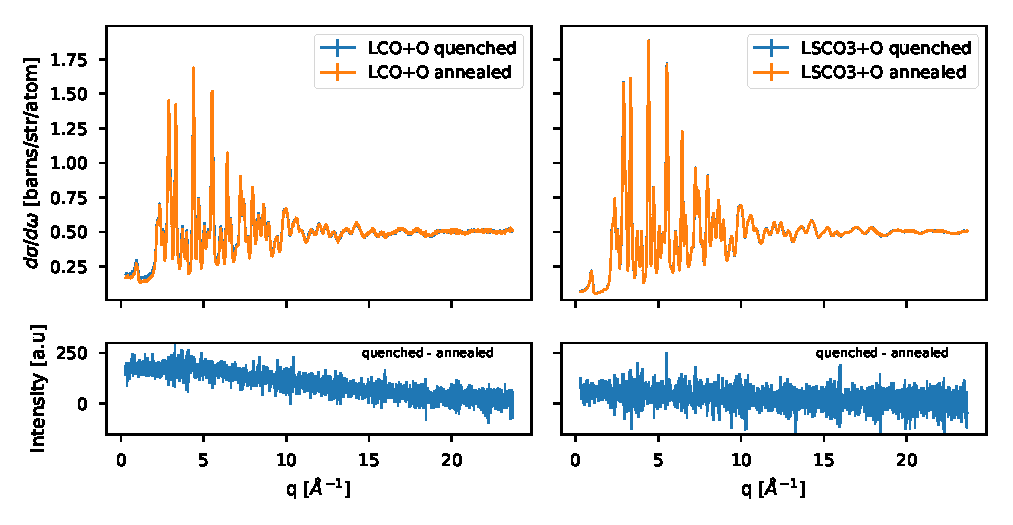
\includegraphics[width=\textwidth]{fig/pdf/quenched_annealed.pdf}
    \caption{Difference between quenched and annealed cooling procedures for LCO+O and LSCO3+O samples. The topmost plots are comparisons of the reduced and corrected $\text{d}\sigma/\text{d}\omega$ in absolute units, while the difference curves are extracted from the raw $\bm{q}$ data.}
    \label{fig:difference}
\end{figure}

\subsection{Sample variation}
In Figure \ref{fig:sample_comparision} we compare the three samples at \SI{300}{\kelvin} in both real and reciprocal space. While the differences are quite small, the difference curves (green) seem to be larger between parent/oxygenated compounds compared to the two oxygenated compounds. This is consistent with a picture where oxygen distorts the lattice in a meaningful way, while the effect of a small amount of strontium is negligible.

\begin{figure}
    \centering
    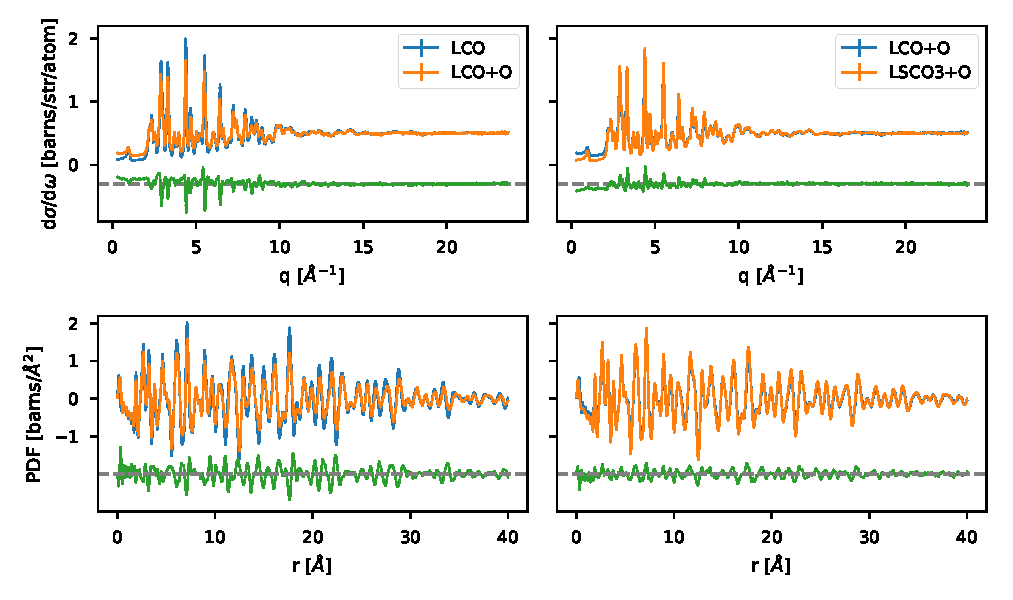
\includegraphics[width=\textwidth]{fig/pdf/sample_comparison.pdf}
    \caption{Comparison of the different samples at \SI{300}{\kelvin} in both real and reciprocal space.}
    \label{fig:sample_comparision}    
\end{figure}

\subsection{Temperature dependence}
Figure \ref{fig:temperature_comparision} shows the high- and low-temperature data for the two oxygen-doped samples. At first glance there seems to be nothing out of the ordinary, peaks are shifting slightly due to thermal expansion (this is particularly easy to spot in the real-space data).

\begin{figure}
    \centering
    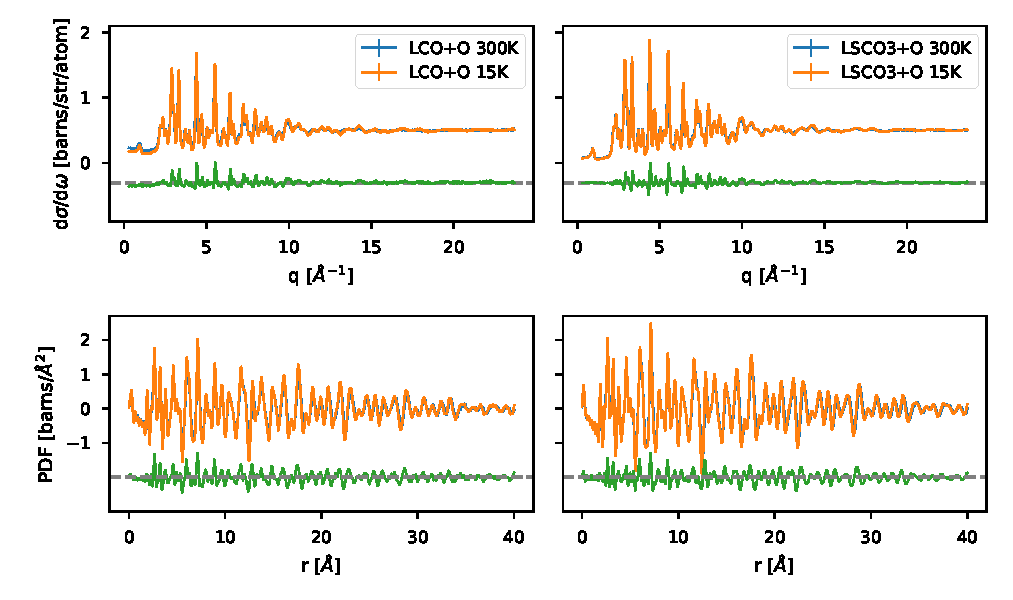
\includegraphics[width=\textwidth]{fig/pdf/temperature_comparison.pdf}
    \caption{Comparison of \SI{300}{\kelvin} and \SI{15}{\kelvin} for LCO+O and LSCO3+O in both real and reciprocal space.}
    \label{fig:temperature_comparision}    
\end{figure}

\subsection{Cu-O distances}
Without performing detailed modelling, we can take a look at the first peak in the real-space data which corresponds to the Cu-O in-plane bond. This bond-length is suspected to be important for superconductivity by controlling the Coulomb interaction (the Hubbard-$U$) \cite{Ivashko2019}. Previously, measurements on La$_{2-x}$Sr$_x$CuO$_{4}$ have shown that the width of the Cu-O bond-length distribution is largest at optimal doping $x=0.15$ and qualitatively tracks the superconducting dome \cite{Bozin2000}. To put this peak into context, we first show the short-range PDF in Figure \ref{fig:medium_range_pdf}. We fit the first peak of all relevant datasets to a single Gaussian as shown in Figure \ref{fig:cu_o_fits} and report the fitting parameters in Table \ref{tab:cu_o_fits}.

Comparing to La$_{2-x}$Sr$_x$CuO$_{4}$, we have roughly the same peak position at $r=\SI{1.9}{\angstrom}$. At \SI{300}{\kelvin} LCO has a smaller width compared to LCO+O and LSCO3+O (within a reasonable certainty). At \SI{15}{\kelvin} the widths are identical to the high-temperature fits (slightly larger but with overlapping errors). Our measurements are thus consistent with the observations of \cite{Bozin2000}.

\begin{figure}
    \centering
    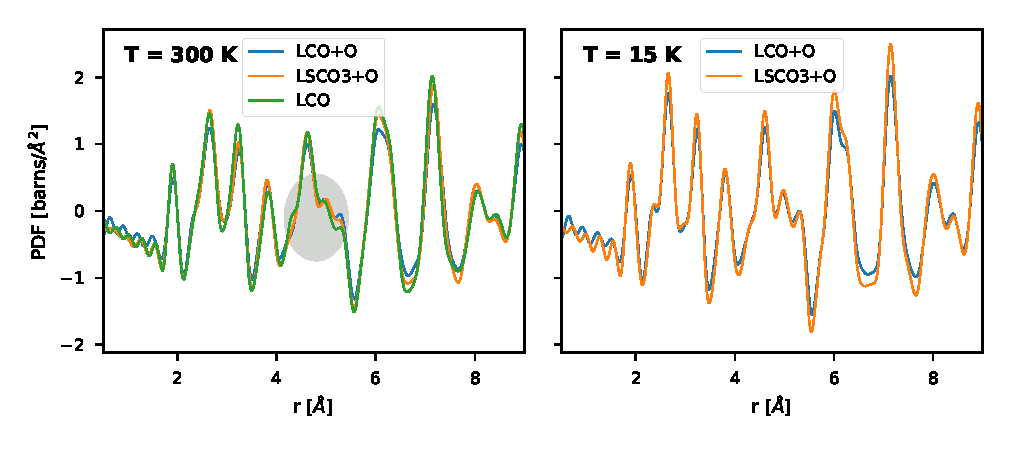
\includegraphics[width=\textwidth]{fig/pdf/medium_range_pdf.pdf}
    \caption{Short range PDF for all samples at \SI{300}{\kelvin} and \SI{15}{\kelvin}.}
    \label{fig:medium_range_pdf}    
\end{figure}

\begin{figure}
    \centering
    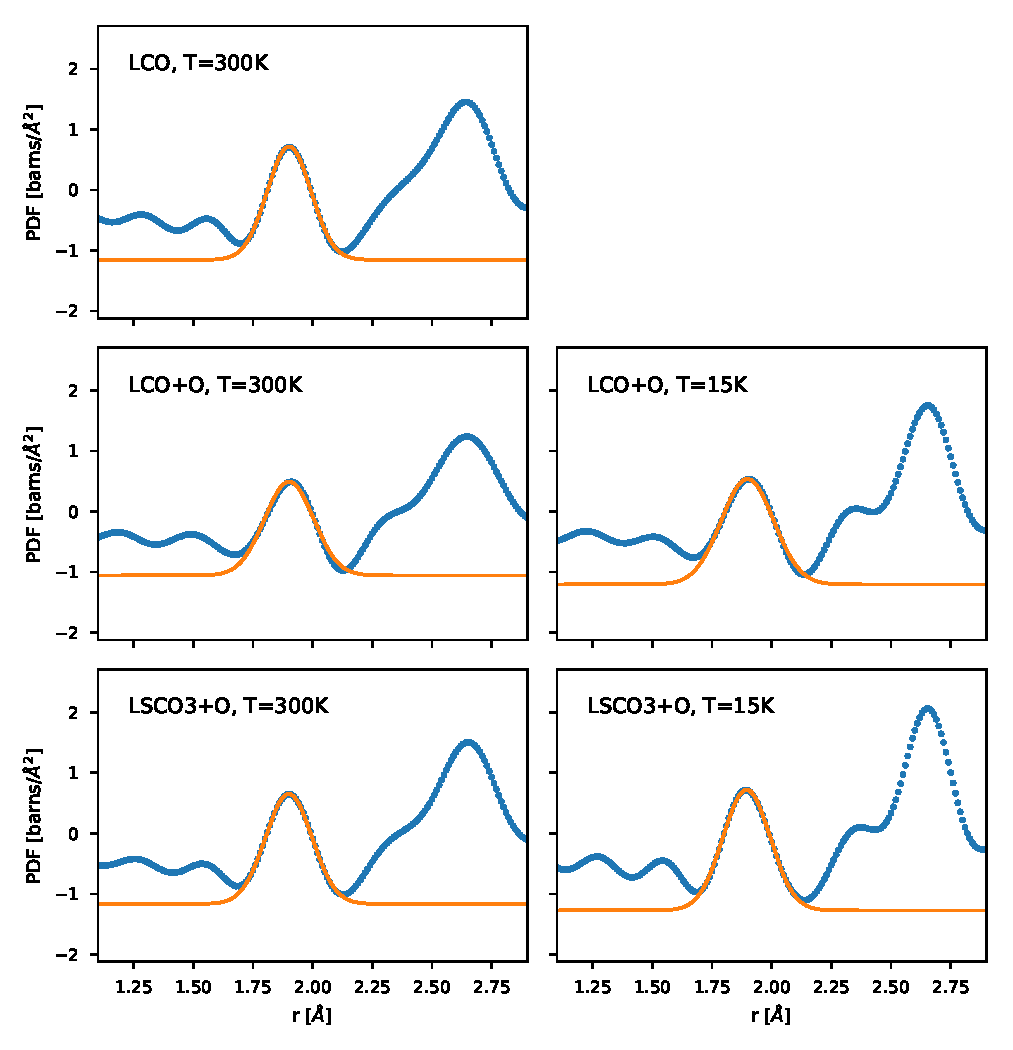
\includegraphics[width=\textwidth]{fig/pdf/cu_o_fits.pdf}
    \caption{Cu-O distance Gaussian fits.}
    \label{fig:cu_o_fits}
\end{figure}

\begin{table}
    \centering
    \begin{tabular}{llll}
        \toprule
          Sample & Temperature [K] &        Cu-O distance [\AA] &           Cu-O $\sigma$ [\AA] \\
        \midrule
             LCO &         300 &  1.9010 $\pm$ 0.0003 &  0.0919 $\pm$ 0.0010 \\
           LCO+O &         300 &  1.9010 $\pm$ 0.0012 &  0.1024 $\pm$ 0.0054 \\
         LSCO3+O &         300 &  1.8995 $\pm$ 0.0003 &  0.0971 $\pm$ 0.0012 \\
           LCO+O &          15 &  1.8983 $\pm$ 0.0009 &  0.1099 $\pm$ 0.0048 \\
         LSCO3+O &          15 &  1.8945 $\pm$ 0.0003 &  0.0987 $\pm$ 0.0012 \\
        \bottomrule
    \end{tabular}    
    \caption{Cu-O distances in all samples at all available temperatures.}
    \label{tab:cu_o_fits}
\end{table}

\subsection{Comparison with simulations}
Finally, in figure \ref{fig:pdf_sim_comparision} I compare LCO and LCO+O at \SI{300}{\kelvin} with molecular dynamics simulations in the LTO phase also at \SI{300}{\kelvin} on an absolute scale with no scaling of either dataset. In general, we seem to have a quite good agreement between the two, especially in the \SIrange{2}{5}{\angstrom} range.

\begin{figure}
    \centering
    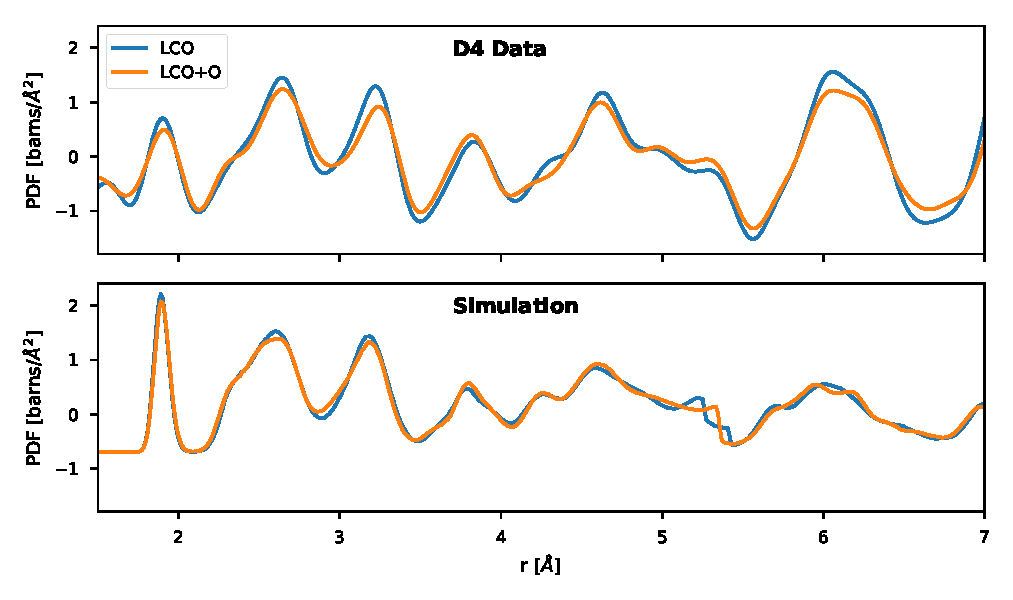
\includegraphics[width=\textwidth]{fig/pdf/pdf_simulation_experiment_compare.pdf}
    \caption[PDF data compared with MD simulation]{PDF data compared with MD simulation}
    \label{fig:pdf_sim_comparision}
\end{figure}